\documentclass[a4paper, 10pt, final, garamond]{book}
\usepackage{cours-preambule}

\makeatletter
\renewcommand{\@chapapp}{Devoir surveill\'e -- révisions}
\makeatother
\renewcommand\thechapter{\!\!}

\begin{document}
\setcounter{chapter}{0}

\def\lspace{25}

\chapter{Commentaires sur le DS de révisions}
\section{Commentaires généraux}

Vous avez donc expérimenté ce que c'est de «~réviser~»… ou pas. Les résultats
sont globalement catastrophiques, les techniques de base du début de l'année
complètement oubliées. Résoudre une équation différentielle~? calculer une
impédance équivalente~? établir la longueur d'équilibre d'un ressort vertical~?
Sans parler de l'optique.

Autrement dit, ne \textbf{tardez pas} à réviser pour de vrai. Suivez mes
recommandations. Bien sûr, il faut vous reposer pendant cet été, mais c'est
\textbf{maintenant} qu'il faut consolider vos acquis. En septembre ça sera trop
tard. Je vous ai indiqué dans la marge deux choses~:
\begin{itemize}
	\item[b]{AR = à revoir} à coté d'une question.
	\item[b]{Détail} s'il faut détailler.
\end{itemize}

\begin{center}
	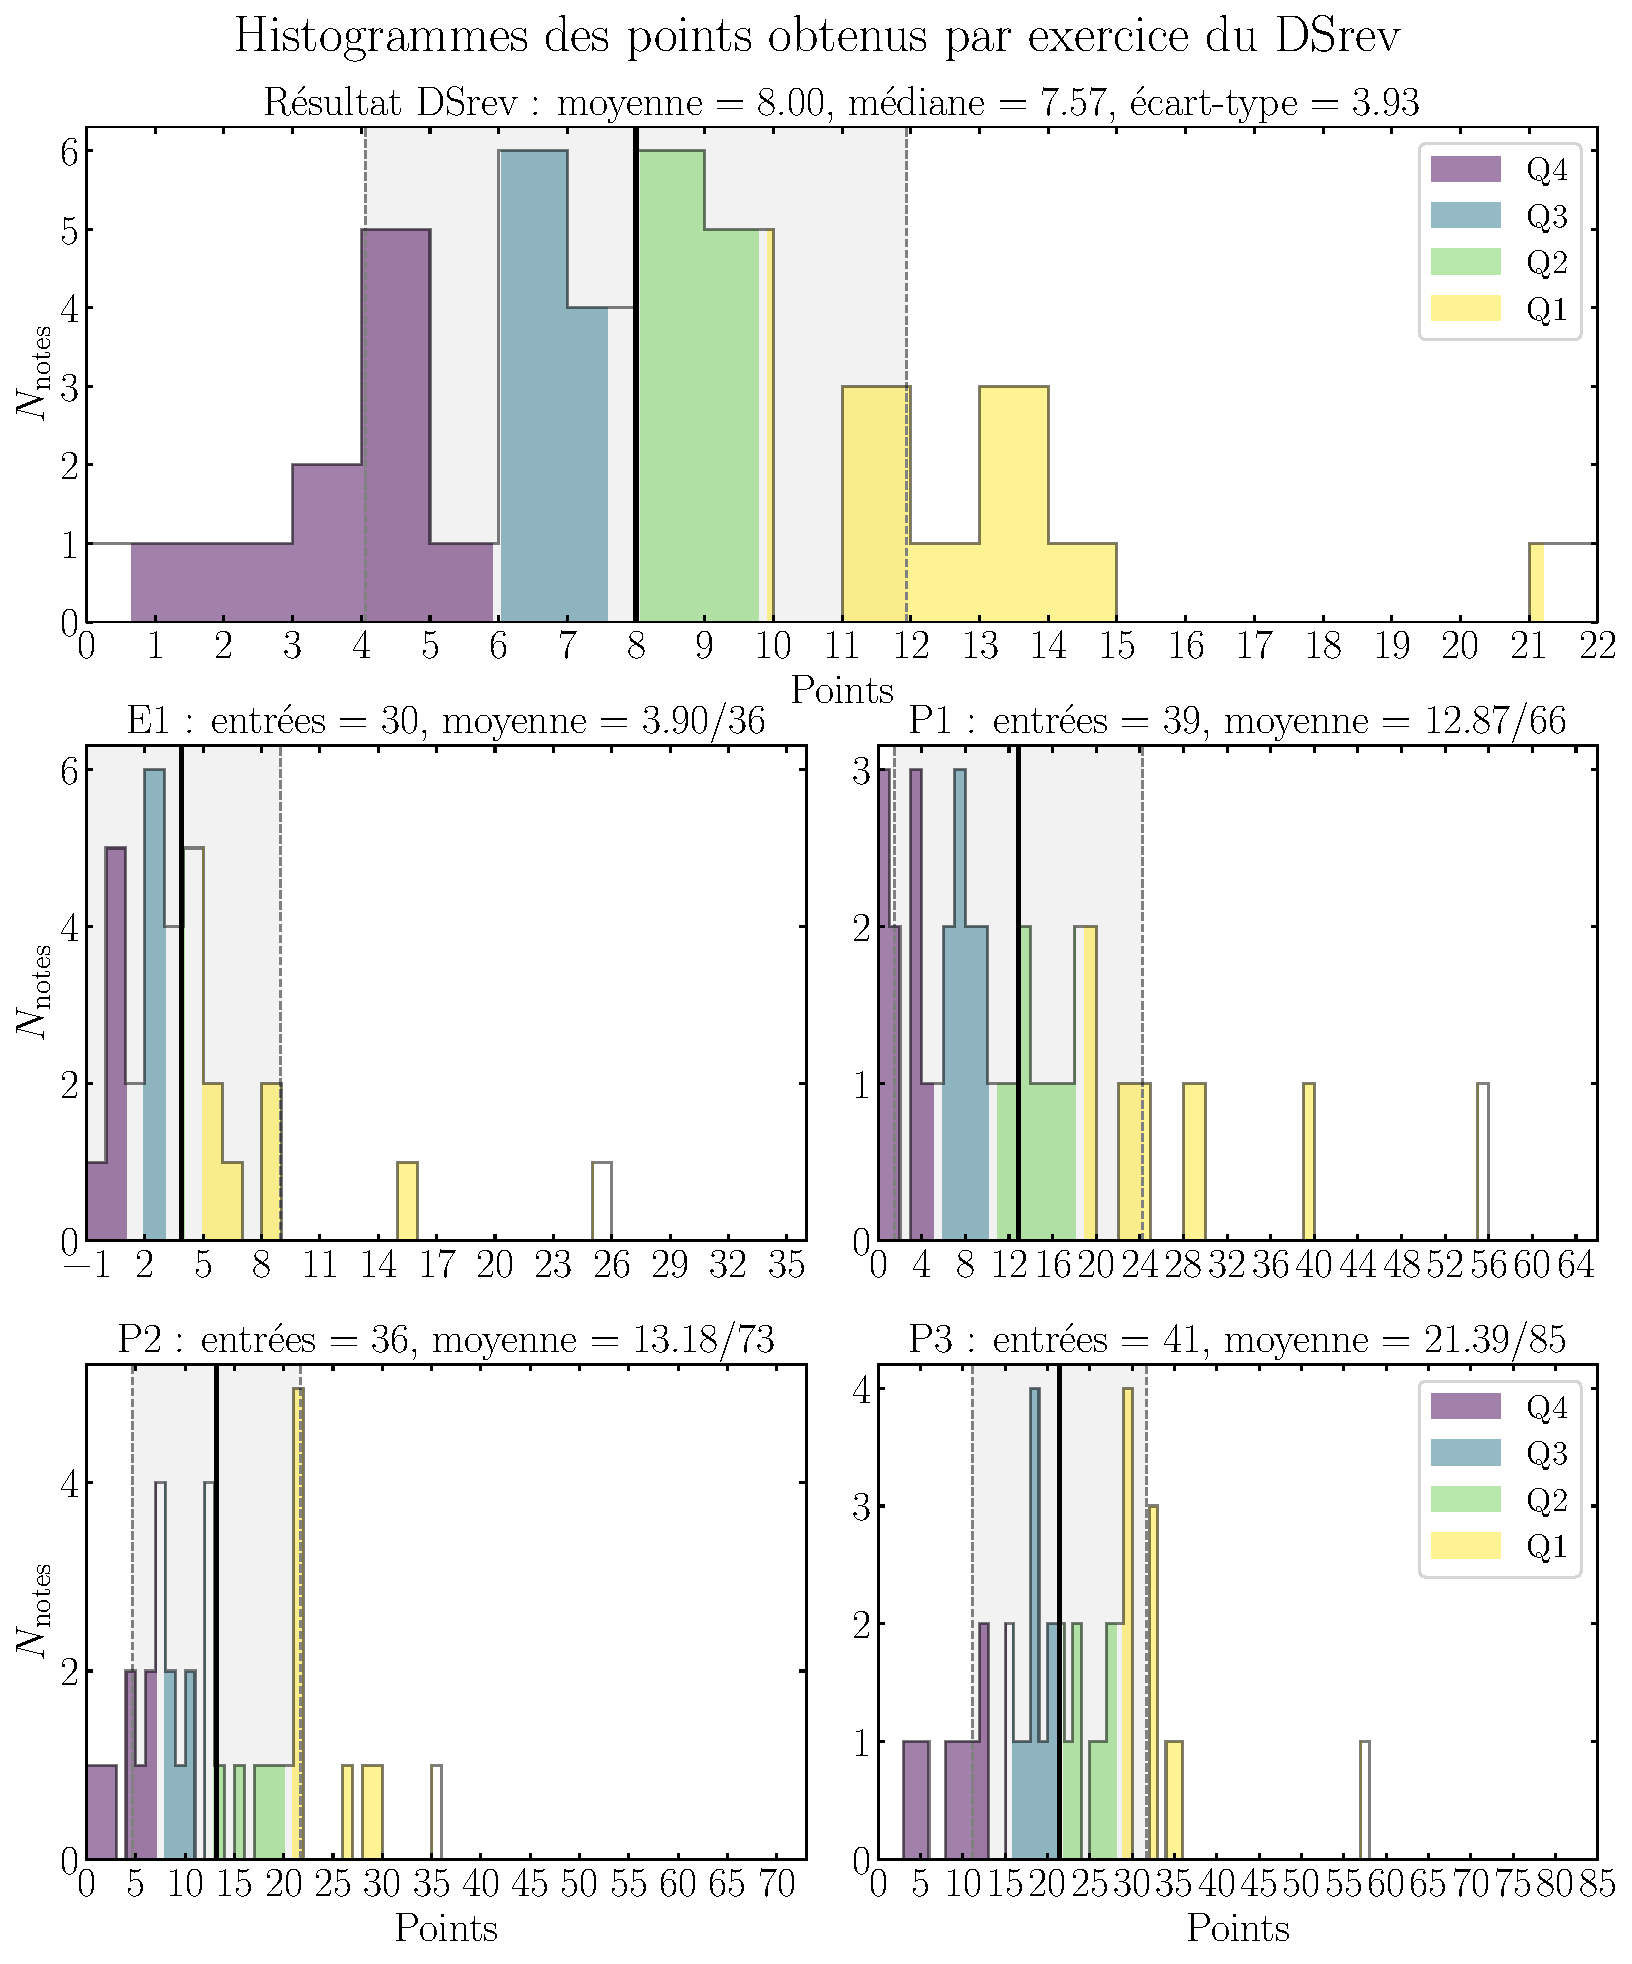
\includegraphics[width=.87\linewidth]{DSrev_hist_all}
\end{center}

\setcounter{section}{0}
\section[36]"E"{Étude d'une lunette de \textsc{Galilée}}
\begin{enumerate}[label=\sqenumi]
	\item[n]{7} % Q1
	N'oubliez pas que les \textbf{distances sont algébriques}~! N'utilisez pas
	des valeurs absolues à tout va.
	\item[n]{8} % Q2
	Cata.
	\item Ah.
	      \smallbreak
	      \begin{enumerate}
		      \item[n]{6} % Q3a
		      \textbf{Les angles sont orientés}~! Il faut savoir gérer les
		      lentilles divergentes…
		      \smallbreak
		      Où sont les schémas optiques
		      $\boxed{\ste(un){\AB}{\infty} \opto{\Lc_1}{O_1}
				      \ABb \opto{\Lc_2}{O_2} \ste(un){\ABp}{\infty}}$~?
		      \item[n]{5} % Q3b
		      Idem, avec les angles orientés il faut savoir exprimer les tangentes
		      selon qu'elles sont négatives ou non.
	      \end{enumerate}
	      \item[n]{9} % Q4
	      Non faite.
	      \item[n]{1} % Q5
	      Non faite.
\end{enumerate}

\setcounter{section}{0}
\section[66]"P"{Filtre linéaire d'ordre 1 et pH-métrie}
Il faut mettre les barres de complexes sous les grandeurs complexes~!
\begin{enumerate}[label=\sqenumi]
	\item[n]{3}  % Q1
	Revoir le placement des fréquences de coupure. 1 seule bonne réponse sur
	toutes les copies…
	\item[n]{8}  % Q2
	Il faut faire les schémas équivalents en BF et HF~!
	\smallbreak
	C'est terriblement triste de voir des «~$i = 0$ donc $u_R = 0$~» alors qu'on a
	deux branches…
	\smallbreak
	Ça fend encore plus le cœur de voir $s(t) \neq 0$ pour un fil, et $s (t) = 0$
	pour un interrupteur ouvert.
	\item[n]{9}  % Q3
	C'est \textbf{gravissime} de ne pas savoir calculer une impédance
	équivalente en parallèle. C'est \textbf{interdit et un blasphème} d'écrire
	quelque chose d'équivalent à $\frac{1}{a+b} = \frac{1}{a} + \frac{1}{b}$.
	\item[n]{4}  % Q4
	Ne pas confondre gain en décibels et gain linéaire.
	\item[n]{8}  % Q5
	Revoir définition pulsation de coupure. \textbf{Ça n'est pas le maximum}.
	\item[n]{16} % Q6
	\textbf{Asymptote $\neq$ limite}~! Ne sautez pas sur $\log H_0 = 0$,
	puisqu'on n'a pas toujours $H_0 = 1$~; ici, $H_0 = \frac{3}{4}$…
\end{enumerate}
\begin{center}
	\begin{framed}
		\Large\bfseries
		Vous ne pouvez pas répondre par un tableau~! On veut voir les asymptotes
		et les équivalents~!!
	\end{framed}
\end{center}
\begin{enumerate}[label=\sqenumi, resume]
	\item[n]{5}  % Q7
	Il faut calculer les coordonnées réelles des points importants pour tracer
	les diagrammes réels.
	\item[n]{13} % Q8
	Il faut retenir le principe d'utilisation des filtres (schéma outil E7.2).
\end{enumerate}

\section[73]"P"{Production de vagues dans une piscine}
\begin{enumerate}[label=\sqenumi]
	\item[n]{2}  % Q1
	Il faut savoir écrire les lettres grecques… $\rho \neq p$.
	\smallbreak
	C'est \textbf{grave} de ne pas connaître la poussée d'\textsc{Archimède}.
\end{enumerate}
\begin{center}
	\begin{framed}
		\Large\bfseries
		$\vv{z}$ n'est pas un vecteur de base~!! $[\vv{z}] = \si{m}$~!! C'est $\uz$
		le vecteur de base~!!
	\end{framed}
\end{center}
\begin{enumerate}[label=\sqenumi, resume]
	\item[n]{12} % Q2
	N'oubliez pas d'établir correctement le système~!
	\smallbreak
	\textbf{Si on vous dit que l'axe est vers le bas, il faut absolument le
		respecter}~!! Sinon toutes les forces et équations sont opposées et c'est un
	enfer à corriger.
	\smallbreak
	\textbf{Refaire le schéma}.
	\smallbreak
	Comment vous faites pour oublier le poids~?
	\item[n]{7}  % Q3
	Des hypothèses très mal gérées.
	\item[n]{4}  % Q4
	Une force de frottement \textbf{s'oppose à la vitesse}, donc $\vv{F}_f =
		-\alpha \dv{z}{t}\uz$~!
	\item[n]{14} % Q5
	Il ne faut pas oublier comment résoudre une équation différentielle d'ordre
	2~!! \textbf{Il y a la solution homogène + la solution particulière~!!}
	\item[n]{9}  % Q6
	Tout est une question de savoir lire une longueur sur un schéma. \textbf{En
		aucun cas une position est une force}. Revoyez absolument cette partie.
	\item[n]{7}  % Q7
	Idem, classique à revoir.
	\item[n]{10} % Q8
	Jamais faite.
	\item[n]{8}  % Q9
	\textbf{Attention} équation très intéressante, puisqu'on cherche le
	\textbf{max} on doit l'exprimer comme un rapport avec le numérateur
	constant, d'où le choix de la question \fbox{8}.
\end{enumerate}

\section[85]"P"{Autour de l'aluminium}
\begin{center}
	\begin{framed}
		\Large
		\bfseries
		Indiquez quand vous répondez sur l'annexe~!! Il faut numéroter les annexes~!
	\end{framed}
\end{center}

\begin{enumerate}[label=\sqenumi]
	\item[n]{6} % Q1
	À revoir.
	\item[n]{5} % Q2
	Bien, mais il faut écrire l'équation dans le bon sens.
	\item[n]{9} % Q3
	Revoir la méthode. \textbf{Commencer par définir $K^\circ$}. Vous pouvez
	travailler sur les potentiels non-multipliés, si vous multipliez votre
	équation en cours de route (ou jouer avec les logarithmes, mais c'est
	risqué).
	\smallbreak
	Les potentiels ont une \textbf{unité}~! Ne vous trompez pas sur la relation de
	\textsc{Nernst}~: c'est $\frac{\ce{Ox}}{\ce{Red}}$ dans le $\log $~! Pensez à
	la relation de \textsc{Henderson} avec $\frac{\text{base}}{\text{acide}}$.
	\item[n]{5} % Q4
	Il faut faire un tableau. \textbf{A pour une intensité j'ai jamais vu ça}. Un
	peu de cohérence quand même.
	\item[n]{7} % Q5
	Peu traitée.
	\item[n]{8} % Q6
	Globalement bien, mais c'est \textbf{illégal} de mettre les acides à haut pH
	et les bases à bas pH.
	\item[n]{5} % Q7
	\textbf{On ne peut \xul{toujours} pas lire un potentiel standard sur les
		diagrammes $E-\pH$}~! Ils dépendent de la convention de tracé.
	\item[n]{3} % Q8
	\item[n]{4} % Q9
	\textbf{Il est grand temps d'intégrer que dans les réactions acide-base,
		\ce{Na^{+}} et \ce{Cl^{-}} sont spectateurs~!!} C'est grave de ne pas savoir
	extraire la réaction acido-basique la plus élémentaire et faite en boucle
	dans tous les TPs depuis la nuit des temps.
	\item[n]{7} % Q10
	Il faut savoir faire la méthode des tangentes.
	\item[n]{4} % Q11
	Bien.
	\item[n]{5} % Q12
	RAS.
	\item[n]{8} % Q13
	Quelques bonnes choses, mais \textbf{attention à la stœchiométrie}.
	\item[n]{2} % Q14
	Non faite.
	\item[n]{3} % Q15
	Non faite.
	\item[n]{4} % Q16
	Non faite.
\end{enumerate}

\end{document}
